%,\documentclass{article}
\documentclass{scrartcl}
\setkomafont{disposition}{\normalfont\bfseries}
\usepackage[utf8]{inputenc}
\usepackage[margin=1in]{geometry}
\usepackage{amsmath}
\usepackage[english]{babel}
\usepackage{mathtools}
\usepackage{amssymb}
\usepackage{amsthm}
\usepackage{breqn}
\usepackage{multicol}
\usepackage{float}
\usepackage{graphicx}
\usepackage{wasysym}
\usepackage{bbold}
\usepackage{hyperref}
\usepackage{enumitem}
\hypersetup{
    colorlinks=true,
    linkcolor=blue,
    filecolor=magenta,      
    urlcolor=cyan,
}
%\pagenumbering{gobble} 
\setlength{\parskip}{1em}
\usepackage[table]{xcolor}
\definecolor{lightgray}{gray}{0.8}
\def\tus{\textunderscore}

\title{Documentation for PopSyCLE}
\subtitle{Population Synthesis for Compact object Lensing Events}
\author{Casey Lam}
\date{September 2019}

\begin{document}

\maketitle

\newpage

\tableofcontents

\newpage
\section{Installation}

\texttt{PopSyCLE} has several dependencies.
In addition to installing \texttt{PopSyCLE}, the user will need \texttt{Galaxia}, \texttt{PopStar}, and several Python libraries.

\subsection{Installing \texttt{Galaxia}}

\subsubsection{Installation}

Note there are also instructions from the creators of \texttt{Galaxia} at \url{http://galaxia.sourceforge.net/Galaxia3pub.html}; what follows is a super pedantic version of that.
\begin{enumerate}
    \item Go to \url{https://sourceforge.net/projects/galaxia/files/} and download \texttt{Galaxia} by clicking the big green button.
    \item Go to your Downloads folder and untar the file by double-clicking it.
    \item Move the untar'd folder (which should be called something like \texttt{galaxia-0.7.2}) to your home directory. 
    (That's the directory where you get sent if you \texttt{cd} and don't put a location. 
    On my laptop, it's $\texttt{/Users/casey/}$).
    \item In your home directory, make a directory called \texttt{GalaxiaData} (i.e. \texttt{mkdir GalaxiaData}).
    \item Move to the \texttt{galaxia-0.7.2} directory (i.e. \texttt{cd galaxia-0.7.2}), and in there, do the following (replacing $\texttt{/Users/casey/}$ with your home directory as appropriate):
    \begin{itemize}
        \item \texttt{./configure --datadir=/Users/casey/GalaxiaData/}
        \item \texttt{make}
        \item \texttt{sudo make install}
        \item \texttt{cp -r GalaxiaData/ /Users/casey/GalaxiaData/}
    \end{itemize}
    \item Move back into your home directory (i.e. \texttt{cd}), then run the following:
    \begin{itemize}
        \item \texttt{galaxia -s warp}
    \end{itemize}
\end{enumerate}
That should be it! 
You don't have to install \texttt{ebf} if you just download \texttt{PopSyCLE}!

NOTE: the instructions in step 5 are assuming a root install. 
If you want to do a local install, you need to have a folder for the software to be installed in.
For example, in my home directory I made a \texttt{sw} directory (\texttt{/Users/casey/sw}) for \texttt{galaxia} to be installed in.
Then I ran the following instead:
    \begin{itemize}
        \item \texttt{./configure --prefix=/Users/casey/sw --datadir=/Users/casey/GalaxiaData/}
        \item \texttt{make}
        \item \texttt{make install}
        \item \texttt{cp -r GalaxiaData/ /Users/casey/GalaxiaData/}
    \end{itemize}
Also, you need to export \texttt{galaxia} to your path. 
In your \texttt{.bash$\_$profile}, add the line \texttt{export PATH=\$PATH:/Users/casey/sw/bin}.
Then proceed with step 6 in the installation instructions.

\subsubsection{Uninstallation}

You need to remove the compiled \texttt{galaxia} code (you can find where it is by typing \texttt{which galaxia} in the terminal), the \texttt{GalaxiaData} directory, and you might as well remove the \texttt{galaxia-0.7.2} directory also.
When you do \texttt{which galaxia} nothing should be returned.

\subsubsection{Parameter modification}

Suppose you want to change the pattern speed in \texttt{Galaxia}.
To do this, follow the installation instructions up to and including step 4.
Then do the following:
\begin{enumerate}
    \item Move to the \texttt{galaxia-0.7.2/src} directory.
    \item Open the \texttt{Population.h} file with your favorite text editor.
    \item Find the pattern speed (in this case by searching for 71.62) and replace with your desired value (in this case 40.00).
    \item Save the change.
\end{enumerate}
Now return to step 5 in the installation instruction and proceed as instructed.

\subsection{Installing \texttt{PopStar}}

\texttt{PopStar} can be installed by cloning the repository from \url{https://github.com/astropy/PopStar}.

\subsection{Installing Python libraries}

We recommend the Anaconda distribution.
In particular, numpy v1.13 or higher is required, along with Astropy and H5py.

\newpage

\section{Reading files}

\texttt{PopSyCLE} use all sorts of different file formats. 
It can easily get confusing, so here is a short guide to the basics.

\subsection{How to read HDF5 files}

Within the HDF5 file are datasets that store the information. It is kind of like a dictionary in python-- the dataset can be manipulated just like a numpy array.

First, go to the directory containing the HDF5 file you want to open. Next, start ipython. Then type the following:

\texttt{import h5py}

\texttt{hf = h5py.File(`filename.h5', `r')}.

If you want to see the names of all the datasets in an HDF5 file, type the following:

\texttt{list(hf.keys())}.

Suppose you want to work with the dataset named \texttt{dname}. 
To access the dataset, type:

\texttt{dset = hf[`dname']}.

Note that only one person at a time can work on an open HDF5 file. Thus, at the end, you need to close the file:

\texttt{hf.close()}.

\subsection{How to read EBF files}

The EBF file is basically a dictionary in python. 
The output of \texttt{Galaxia} is in the EBF format. 

First, go to the directory containing the EBF file you want to open. 
Next, start ipython. 
Then type the following:

\texttt{import ebf}

\texttt{ef = ebf.read(`filename.ebf', `/')}.

If you want to see the names of all the keys in the EBF file, type the following:

\texttt{ef.keys()}.

Suppose you want to work with the key \texttt{xkey}. To access that part of the file, type:

\texttt{x = ef[`xkey']}.

Now \texttt{x} is just a numpy array and can manipulated as such.

\subsection{How to read FITS table files}

First, go to the directory containing the fits file you want to open. Next, start ipython, Then type the following:

\texttt{from astropy.table import Table}

\texttt{tab = Table.read(`table.fits')}

To view the entire table, just type \texttt{tab}. The table works similar to a python dictionary. 
The column names are the keys of the dictionary, and the dictionary name in this case is \texttt{tab}.

To view the header information/metadata, type

\texttt{tab.meta}.

\newpage 

\section{Description of Pipeline}

First, run \texttt{Galaxia} to create an EBF file, which produces a synthetic survey, i.e. a bunch of stars.
Next, run population synthesis (perform\tus pop\tus syn) to inject compact objects into the synthetic survey; both the compact objects and stars are saved in an HDF5 file.
Then run a synthetic survey (calc\tus events and refine\tus events) that will produce a list of microlensing events, which are listed in a FITS file.
\begin{figure}[h]
    \centering
    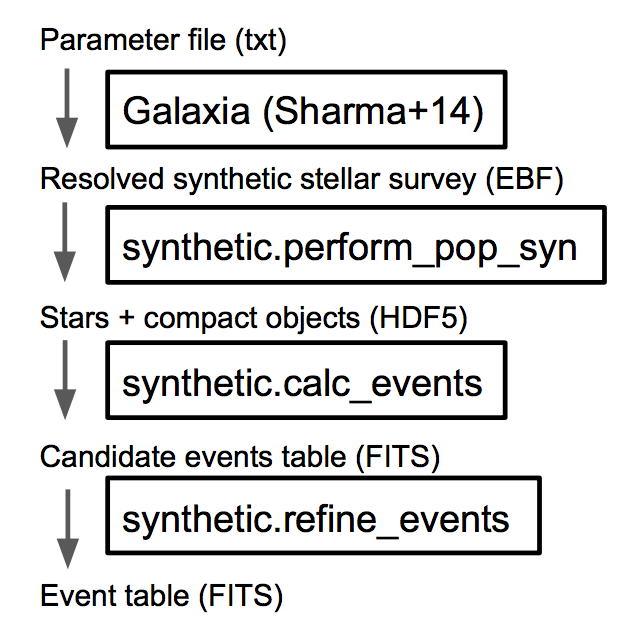
\includegraphics[scale=0.7]{pipeline.png}
    \caption{Flowchart of pipeline.}
\end{figure}

\newpage

\section{Outputs}

In addition to the outputs about to be described, each function produces a text log file that lists the input parameters.

\subsection{perform\tus pop\tus syn}

\subsubsection{Label/summary file (Astropy FITS table)}

\begin{itemize}
    \item file$\_$name is the name of the dataset for the HDF5 file.
    
    \item long$\_$start and long$\_$end are the edges of the longitude bin.
    
    \item lat$\_$start and lat$\_$end are the edges of the latitude bin.
    
    \item objects is the number of objects in that latitude/longitude bin.
    
    \item N$\_$stars, N$\_$WD, N$\_$NS, and N$\_$BH are the number of stars, white dwarfs, neutron stars, and black holes, respectively, in that latitude/longitude bin. 
    The sum of these should be equal to the total number of objects.
\end{itemize}
Total white dwarfs is equal to adding the numbers of WDs made from MIST and the IFMR. 
WDs from the MIST models have photometry (they're bright), while WDs from the IFMR and are dark (roughly 30th magnitude and below, so we assign them a value of \texttt{nan} for their magnitude.)

\begin{figure}[h]
    \centering
    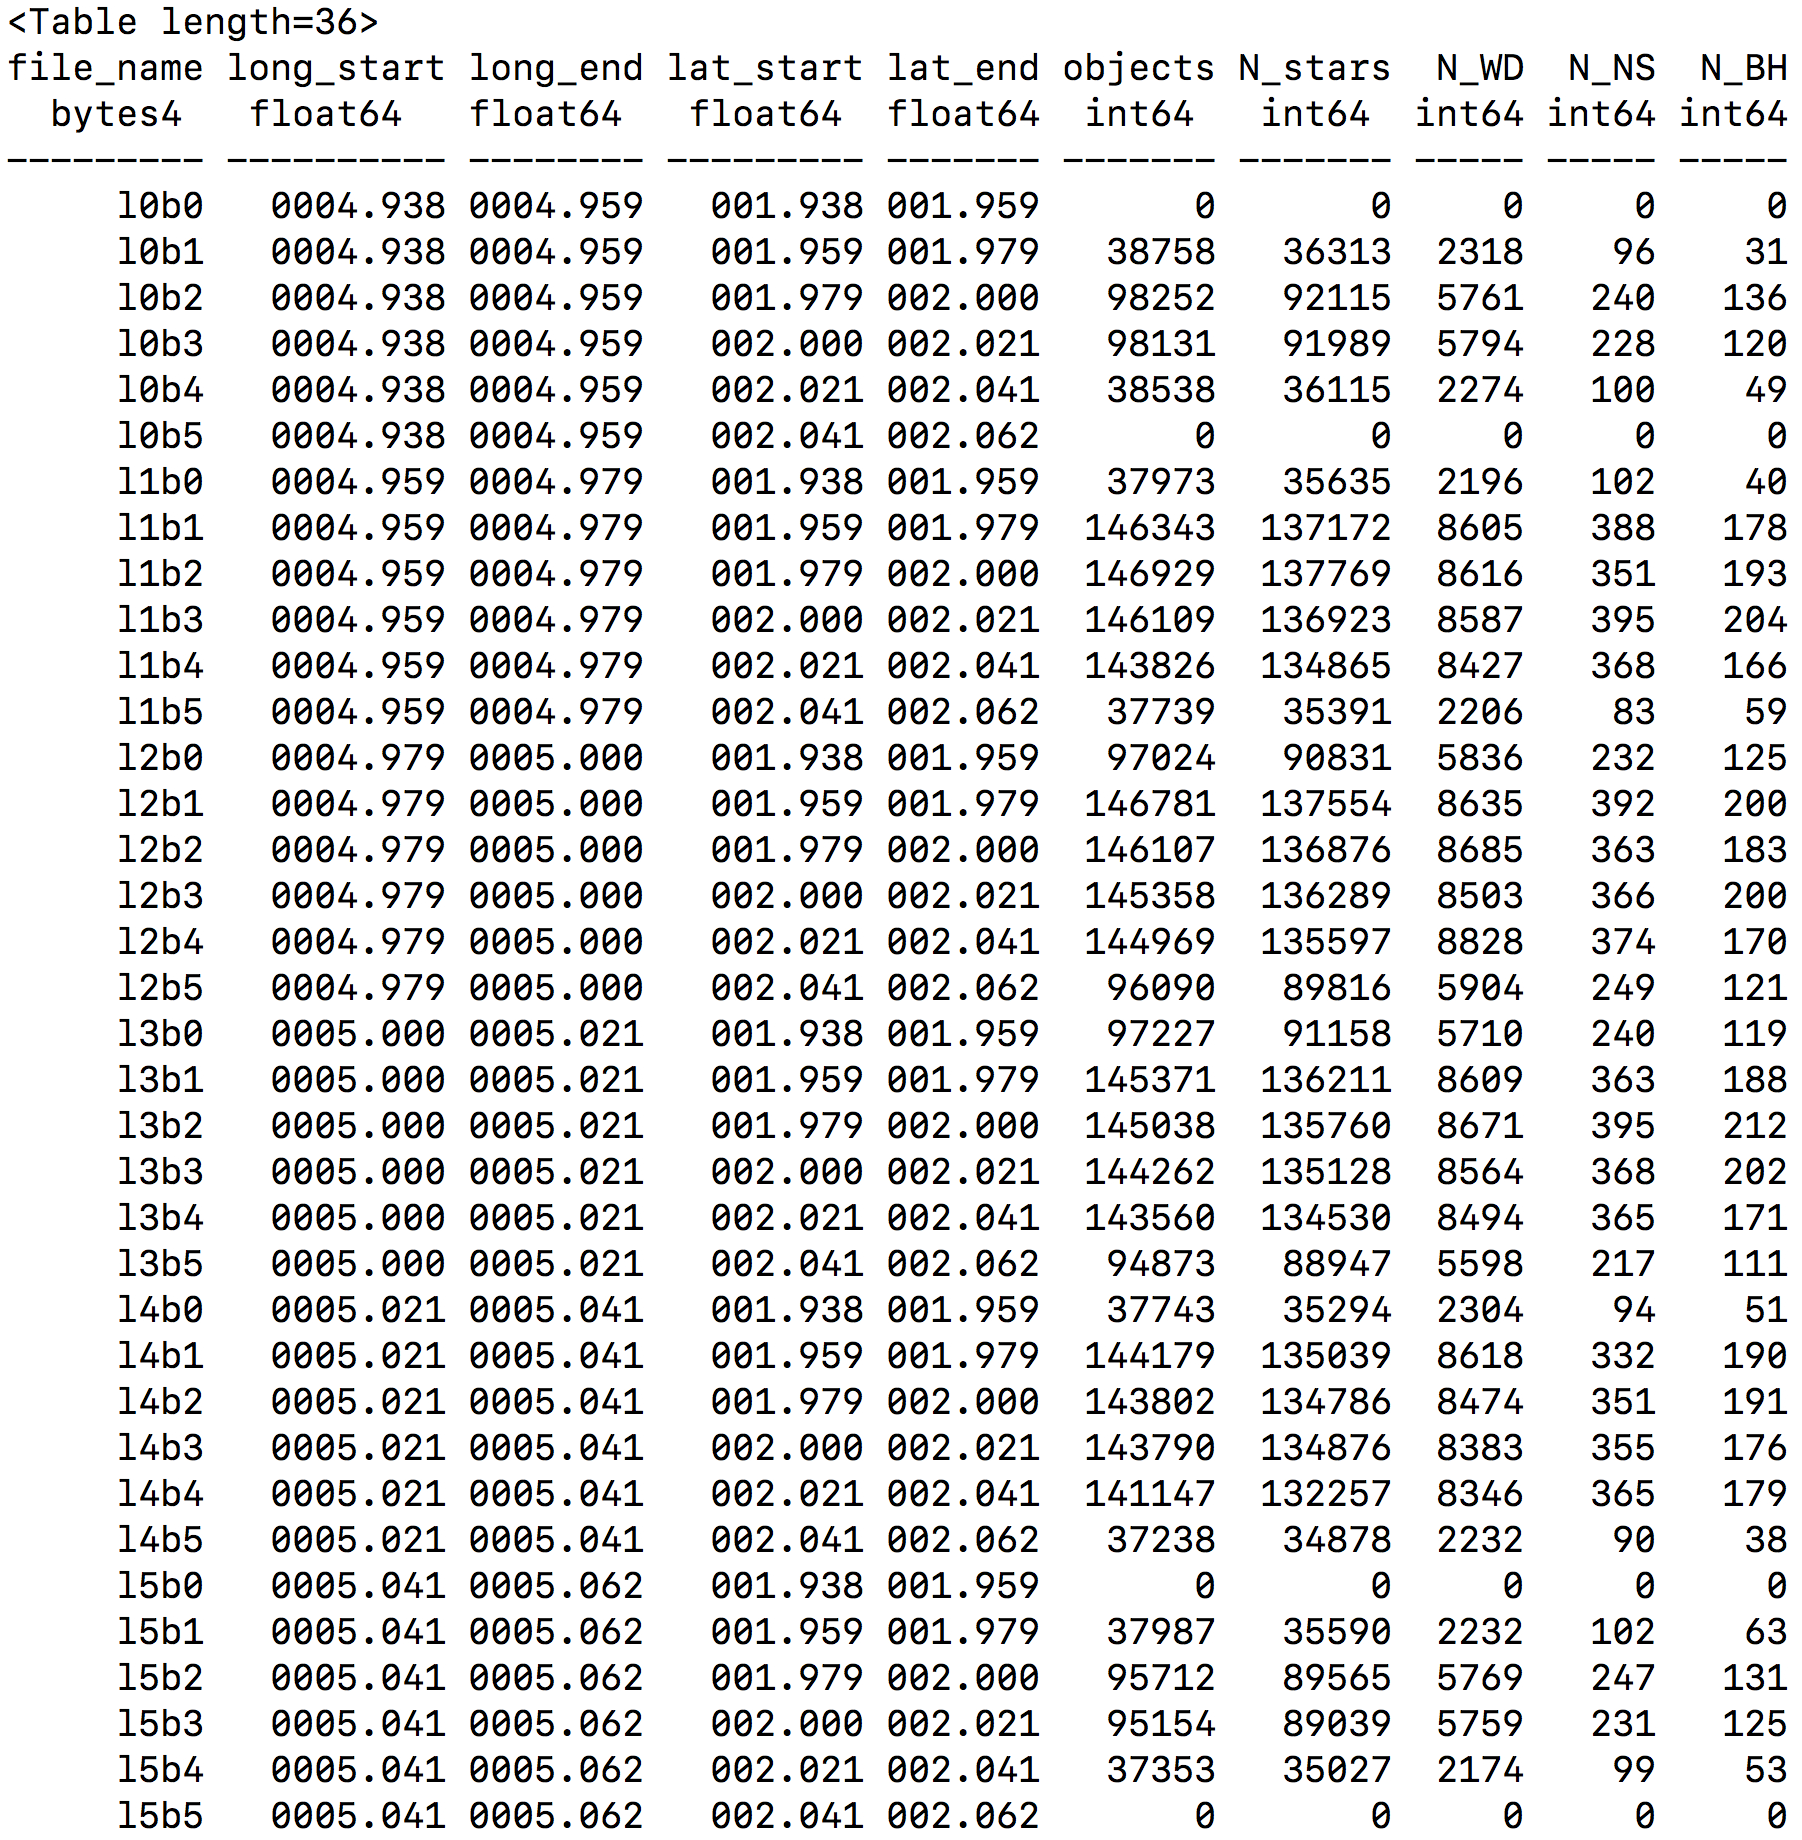
\includegraphics[scale=0.3]{fits.png}
\end{figure}

\newpage 

\subsubsection{Stars and compact objects (HDF5)}

The data output contained in the HDF5 datasets are a combination of outputs that come directly from Galaxia, and outputs we ourselves have calculated or defined.

\begin{table}[h]
\centering
\rowcolors{1}{white}{lightgray}
\begin{tabular}{ l | l | p{6.5cm} | l }
    \textbf{Index} & \textbf{Tag name} & \textbf{Brief Description} & \textbf{Units} \\ 
    \hline
    $[0]$ & zams$\_$mass & ZAMS mass & $M_\odot$ \\ 
    $[1]$ & rem$\_$id & Integer indicating the remnant object type (more details in tag description) & N/A \\
    $[2]$ & mass & Current mass & $M_\odot$ \\
    $[3]$ & px & Heliocentric x position & kpc \\
    $[4]$ & py & Heliocentric y position & kpc \\
    $[5]$ & pz & Heliocentric z position & kpc \\
    $[6]$ & vx & Heliocentric x velocity & km/s \\
    $[7]$ & vy & Heliocentric y velocity & km/s \\
    $[8]$ & vz & Heliocentric z velocity & km/s \\
    $[9]$ & rad & Galactic radial distance & kpc \\
    $[10]$ & glat & Galactic latitude & deg \\
    $[11]$ & glon & Galactic longitude & deg \\
    $[12]$ & vr & Galactic radial velocity & km/s \\
    $[13]$ & mu$\_$b & Galactic proper motion, b component  & mas/yr \\
    $[14]$ & mu$\_$lcosb & Galactic proper motion, l component & mas/yr \\
    $[15]$ & age & Age & log(age/yr) \\
    $[16]$ & popid & Population ID-- integer indicating the population type ranging from 0 to 9 & N/A \\
    $[17]$ & ubv$\_$k & UBV photometric system, K-band absolute magnitude & mag \\
    $[18]$ & ubv$\_$i & UBV photometric system, I-band absolute magnitude & mag \\
    $[19]$ & exbv & Extinction E(B-V) at the location of star given by 3-D Schlegel extinction maps & mag \\
    $[20]$ & obj$\_$id & Object ID-- unique integer to identify star/compact object & N/A \\
    $[21] - [26]$ & ubv$\_$j, u, r, b, h, v & UBV photometric system, J, U, R, B, H, V absolute magnitude (in this order) & mag \\
    $[27]$ & teff & Effective temperature & log(T/Kelvin) \\
    $[28]$ & grav & Surface gravity & log(gravity) \\
    $[29]$ & mbol & Bolometric magnitude & log(L/$L_\odot$) \\
    $[30]$ & feh & Metallicity & $[Fe/H]$ \\
\end{tabular}
\caption{ Note that the tag names are NOT used in the HDF5 files. 
They are just listed here to show the direct correspondence between the HDF5 outputs and the Astropy table of candidate events (next section.) }
\end{table}

For stars (which are generated by Galaxia), the following outputs are taken directly from Galaxia and just reformatted into the HDF5 format; parenthetical names correspond to the tag name from Galaxia, if different: zams$\_$mass (smass), mass (mact), px, py, pz, vx, vy, vz, age, popid, ubv$\_$k, ubv$\_$i, ubv$\_$u, ubv$\_$b, ubv$\_$v, ubv$\_$r, ubv$\_$j, ubv$\_$h, exbv (exbv$\_$schlegel), teff, grav, mbol (lum), feh. Note that the lum key from Galaxia is referred to as mbol in the Galaxia documentation.
For compact objects (which we generated with our population synthesis code), we must assign these values ourselves. 
For both stars and compact objects, the following are things we have directly calculated or assigned ourselves: rem$\_$id, rad, glat, glon, vr, mu$\_$b, mu$\_$lcosb, obj$\_$id.\footnote{For reasons relating to managing RAM, we calculate rad, glat, and glon although they are an output given directly from Galaxia, and we could have just read in the value. 
However, it can be calculated directly from knowledge of px, py, and pz.}

\newpage

\subsection{calc\tus events}

\subsubsection{Event candidates table (Astropy FITS table)}

The event candidates table is very similar to the HDF5 file created in perform\tus pop\tus syn.
(In fact, the top part is completely duplicated; it's here for completeness.) 
However, the main difference is that there is a LOT less of the output, so instead of writing it in arrays in an HDF5 file, we use an Astropy table.

\begin{table}[h]
\centering
\rowcolors{1}{white}{lightgray}
\begin{tabular}{ l | p{6.5cm} | p{3cm} }
    \textbf{Tag name} & \textbf{Brief Description} & \textbf{Units}  \\
    \hline
    zams$\_$mass ($\_$L, $\_$S) & ZAMS mass & $M_\odot$ \\
    rem$\_$id ($\_$L, $\_$S) & Remnant ID-- integer indicating the remnant object type ranging from 0 to 3 & N/A \\
    mass ($\_$L, $\_$S) & Current mass & $M_\odot$ \\
    px ($\_$L, $\_$S) & Heliocentric x position & kpc \\
    py ($\_$L, $\_$S) & Heliocentric y position & kpc \\
    pz ($\_$L, $\_$S) & Heliocentric z position & kpc \\
    vx ($\_$L, $\_$S) & Heliocentric x velocity & km/s \\
    vy ($\_$L, $\_$S) & Heliocentric y velocity & km/s \\
    vz ($\_$L, $\_$S) & Heliocentric z velocity & km/s \\
    rad ($\_$L, $\_$S) & Galactic radial distance & kpc \\
    glat ($\_$L, $\_$S) & Galactic latitude b & deg \\
    glon ($\_$L, $\_$S) & Galactic longitude l & deg \\
    vr ($\_$L, $\_$S) & Galactic radial velocity & km/s \\
    mu$\_$b ($\_$L, $\_$S) & Galactic proper motion, b component & mas/yr \\
    mu$\_$lcosb ($\_$L, $\_$S) & Galactic proper motion, l component & mas/yr \\
    age ($\_$L, $\_$S) & Age & log(age/yr) \\
    popid ($\_$L, $\_$S) & Population ID-- integer indicating the population type ranging from 0 to 9 & N/A \\
    ubv$\_$u, b, v, i, r, j, h, k ($\_$L, $\_$S) & UBV photometric system absolute magnitudes & mag \\
    exbv ($\_$L, $\_$S) & Extinction E(B-V) at the location of star given by 3-D Schlegel extinction maps & mag \\
    obj$\_$id ($\_$L, $\_$S) & Object ID-- unique integer to identify star/compact object & N/A \\
    teff ($\_$L, $\_$S) & Effective temperature & log(T/Kelvin) \\
    grav ($\_$L, $\_$S) & Surface gravity & log(gravity) \\
    mbol ($\_$L, $\_$S) & Bolometric magnitude & log(L/$L_\odot$) \\
    feh ($\_$L, $\_$S) & Metallicity &  $[Fe/H]$\\
    theta$\_$E & (Angular) Einstein radius & mas \\
    mu$\_$rel & Relative source-lens proper motion & mas/yr \\
    u0 & (Unitless) minimum source-lens separation, \emph{during} the survey & dim'less (normalized to $\theta_E$) \\
    t0 & Time at which minimum source-lens separation occurs & days
\end{tabular}
\end{table}
Tag names ARE used for the Astropy table. You will see a lot of the tag names have a parenthetical after ($\_$L, $\_$S). That is to indicate there is one tag for the lens (L) and one for the source (S), since for a given event, you need to have both a lens and a source, and each of these things has a mass, a velocity, a position, etc. For example, zams$\_$mass$\_$L is the ZAMS mass of the lens, and age$\_$S is the log(age/yr) of the source. 

\subsubsection{Blends table (Astropy FITS table)}

For each candidate microlensing event, associated with it are blended stars, which we call neighbors.
Given the blend radius chosen when running calc\tus events, the blend table saves all neighbor stars that fall within that distance from the lenses in the candidate events table.
The blends table is again almost identical to the HDF5 output, but is has three additional items.
For each neighbor star, it lists the object ID of the lens and source it is associated with, and the distance between itself and the lens.
Note that there can be multiple neighbor stars associated with a single lens and source (microlensing event).

\begin{table}[h]
\centering
\rowcolors{1}{white}{lightgray}
\begin{tabular}{ l | p{6.5cm} | p{3cm} }
    \textbf{Tag name} & \textbf{Brief Description} & \textbf{Units}  \\
    \hline
    zams$\_$mass$\_$N & ZAMS mass & $M_\odot$ \\
    rem$\_$id$\_$N & Remnant ID-- integer indicating the remnant object type ranging from 0 to 3 & N/A \\
    mass$\_$N & Current mass & $M_\odot$ \\
    px$\_$N & Heliocentric x position & kpc \\
    py$\_$N & Heliocentric y position & kpc \\
    pz$\_$N & Heliocentric z position & kpc \\
    vx$\_$N & Heliocentric x velocity & km/s \\
    vy$\_$N & Heliocentric y velocity & km/s \\
    vz$\_$N & Heliocentric z velocity & km/s \\
    rad$\_$N & Galactic radial distance & kpc \\
    glat$\_$N & Galactic latitude b & deg \\
    glon$\_$N & Galactic longitude l & deg \\
    vr$\_$N & Galactic radial velocity & km/s \\
    mu$\_$b$\_$N & Galactic proper motion, b component & mas/yr \\
    mu$\_$lcosb$\_$N & Galactic proper motion, l component & mas/yr \\
    age$\_$N & Age & log(age/yr) \\
    popid$\_$N & Population ID-- integer indicating the population type ranging from 0 to 9 & N/A \\
    ubv$\_$u, b, v, i, r, j, h, k$\_$N & UBV photometric system absolute magnitudes & mag \\
    exbv$\_$N & Extinction E(B-V) at the location of star given by 3-D Schlegel extinction maps & mag \\
    obj$\_$id$\_$N & Object ID-- unique integer to identify star/compact object & N/A \\
    teff$\_$N & Effective temperature & log(T/Kelvin) \\
    grav$\_$N & Surface gravity & log(gravity) \\
    mbol$\_$N & Bolometric magnitude & log(L/$L_\odot$) \\
    feh$\_$N & Metallicity &  $[Fe/H]$\\
    obj$\_$id$\_$L & Object ID of the lens & N/A \\
    obj$\_$id$\_$S & Object ID of the source & N/A \\
    sep$\_$LN & Separation between lens and neighbor & arcsec 
\end{tabular}
\end{table}

\newpage 

\subsection{refine\tus events}

\subsubsection{Events table (Astropy FITS table)}

The output here is very similar to the candidate events table.
In fact, part of it is completely duplicated.
All tags listed in the event candidates table are also part of the events table.
However, the following columns are also appended. 
NOTE: the entries for u0 and t0 are \emph{overwritten}; the values for u0 and t0 returned from calc$\_$events is different from that returned in refine$\_$events.
Each refine\tus events file requires you to choose a filter and extinction law; in this table we suppose filter $x$ is chosen.
\begin{table}[h]
\centering
\rowcolors{1}{white}{lightgray}
\begin{tabular}{ l | p{6.5cm} | p{3cm} }
    \textbf{Tag name} & \textbf{Brief Description} & \textbf{Units}  \\
    \hline
    u0 & (Unitless) minimum source-lens separation, \emph{during} the survey & dim'less \\
    t0 & Time at which minimum source-lens separation occurs & days \\
    delta$\_$m$\_x$  & Bump amplitude (difference in baseline and maximum magnification magnitude) in $x$-band & mag \\
    pi$\_$rel & Relative parallax & mas \\
    pi$\_$E & Microlensing parallax & dim'less \\
    t$\_$E & Einstein crossing time & days \\
    ubv$\_x\_$app ($\_$L, $\_$S) & UBV photometric system, $x$-band apparent magnitude, with extinction & mag \\
    ubv$\_x\_$LSN & Blended magnitude in $x$  band (Apparent magnitude of source + lens + neighbors) & mag\\
    f$\_$blend$\_x$  & Source flux fraction (unlensed source flux divided by baseline) in $x$-band & dim'less \\
    cent$\_$glon$\_x\_$N & Galactic longitude l of neighbor stars' centroid & deg \\
    cent$\_$glat$\_x\_$N & Galactic latitude b of neighbor stars' centroid & deg\\
    ubv$\_x\_$app$\_$N &  Apparent magnitude of neighbor stars, $x$-band apparent magnitude & mag\\
\end{tabular}
\end{table}

\newpage

\newpage

\subsection{Additional descriptions of tags}
\begin{description}
    \item [rem$\_$id] These label the different types of remnant objects (star, black hole, neutron star, or white dwarf.) They are identified as following:
    \begin{itemize}
        \item 0: Star
        \item 101: WD 
        \item 102: NS
        \item 103: BH
    \end{itemize}
    
    \item [popid] Describes which population is generated.\footnote{In \texttt{Galaxia} there is an option for a 10th population type; the Bullock and Johnston stellar halos. We have chosen not use it, and the code is not written to include it.} They are identified as following:
    \begin{itemize}
        \item 0: Thin disk, $\leq$ 0.15 Gyr
        \item 1: Thin disk, 0.15-1 Gyr
        \item 2: Thin disk, 1-2 Gyr
        \item 3: Thin disk, 2-3 Gyr
        \item 4: Thin disk, 3-5 Gyr
        \item 5: Thin disk, 5-7 Gyr
        \item 6: Thin disk, 7-10 Gyr
        \item 7: Thick disk, 11 Gyr (single-age)
        \item 8: Stellar halo, 14 Gyr (single-age)
        \item 9: Bulge, 10 Gyr (single-age)
    \end{itemize}
    
    \item [px, py, pz; vx, vy, vz] These are given in heliocentric coordinates (i.e. Cartesian coordinates with the sun at the origin.) See subsection on coordinate systems for more information.
    
    \item [rad, glat, glon; vr, mu$\_$b, mu$\_$lcosb] These are given in galactic coordinates (i.e. spherical coordinates with the sun at the origin.) See subsection on coordinate systems for more information.
    
    \item [ubv$\_$u, b, v, r, i, j, h, k; exbv] Photometry information is given in absolute magnitude. For NSs and BHs, all these values are \texttt{nan} to indicate they are dark.
    
    \item [t0] Note that you can have a negative day (this just means time before the ``zero" time, which is defined as the state of the system that is generated by Galaxia and the population synthesis. Since we are assuming everything moves in straight lines, we can propagate either forward or backwards.
 \end{description}

\newpage
 
\section{Coordinates Systems} 
There are two different coordinate systems used, Heliocentric and Galactic. 
Heliocentric coordinates are Cartesian coordinates with the sun at the origin. The positive $x$ axis is pointing toward the Galactic Center, and the positive $z$ axis is pointing toward the Galactic North Pole.
Galactic coordinates are spherical coordinates with the sun at the origin. 
Longitude $l$ is measuring the angular distance of an object eastward along the galactic equator from the galactic center, and latitude $b$ is measuring the angle of an object north or south of the galactic equator (or midplane) as viewed from Earth; positive to the north, negative to the south. 
Radius $r$ is the distance from the sun to the object. 

The conversion between Heliocentric and Galactic is just the same as converting between rectangular to spherical coordinates, where $\phi = l$ and $\theta = -b + 90^\circ$.
Going from Galactic to Heliocentric (units are degrees):
\begin{align*}
    x &= r \mathrm{sin}(-b + 90^\circ) \mathrm{cos}l =  r \mathrm{cos}b \mathrm{cos}l  \\
    y &= r \mathrm{sin}(-b + 90^\circ) \mathrm{sin}l = r \mathrm{cos}b \mathrm{sin}l \\
    z &= r \mathrm{cos}(-b + 90^\circ) = r \mathrm{sin}b
\end{align*}

Going from Heliocentric to Galactic (units are degrees):
\begin{align*}
    r &= \sqrt{x^2 + y^2 + z^2} \\
    b &= -\mathrm{cos}^{-1}(z/r) + 90^\circ \\
    l &= \mathrm{tan}^{-1}(y/x)
\end{align*}
Note: be careful with the branch of arctangent. Practically, use \texttt{numpy.arctan2} if using Python.

\begin{figure}[h]
    \centering
    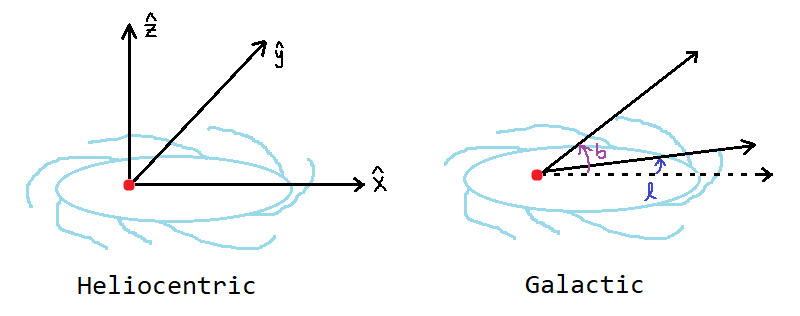
\includegraphics[scale=0.7]{coords.png}
    \caption{Diagram of Heliocentric and Galactic coordinate systems. The red dot is the sun.}
\end{figure}

% \newpage

% \section{Example: Calculating an Einstein crossing time distribution}
% Here we run an example, start to finish, on how to calculate an Einstein crossing time distribution.

% \subsection{Generating synthetic stellar survey with Galaxia}
% \begin{itemize}
%     \item Create/edit parameter file (briefly describe parameters)
%     \item galaxia -r parameterfile
% \end{itemize}

% \subsection{Population synthesis}
% \begin{itemize}
%     \item Run perform\tus pop\tus syn
% \end{itemize}

% \subsection{Event candidate calculation}
% \begin{itemize}
%     \item Run calc\tus events
% \end{itemize}

% \subsection{Event selection}
% \begin{itemize}
%     \item Run refine\tus events
% \end{itemize}

% \newpage

% \section{Additional References}

% \subsection{Galaxia and EBF}

% \begin{itemize}
%     \item Galaxia Paper: \href{http://iopscience.iop.org/article/10.1088/0004-637X/730/1/3/meta}{On IOP Science}
%     \item Galaxia download and documentation: \href{http://galaxia.sourceforge.net/}{SourceForge site}
%     (Note: site often randomly under maintenance.)
%     \item Presentation about EBF: \href{https://www.atnf.csiro.au/research/WALLABY/Wallaby2011/SIM-FEST2011-SSharma.pdf}{Slides by Sanjib Sharma}
% \end{itemize}

% \section{Miscellaneous}

% \subsection{Random seed in \texttt{Galaxia}}

\end{document}
